\chapter{Basic Tools} \label{ch:numpyscipy}

Python has been increasingly popular for data science in the past few years. Many libraries and tools have been developed for Python to enhance its data analysis and visualization capabilities, just to name a few, \verb|numpy|, \verb|scipy|, \verb|scikit-learn|, \verb|pandas|, \verb|matplotlib| \verb|tensorflow| and \verb|pytorch|.

This chapter together with a few consequent chapters introduces commonly used tools that data science adopts using Python. This part of the notebook is more application driven, and only the basic implementations are introduced. We are not digging into the theory supporting machine learning and artificial intelligence.

It has been increasingly popular today to use Python together with Conda and jupyter-lab/jupyter notebook. Conda is an open-source language-agnostic package and environment management system. Jupyter notebook is an interactive computing platform for Python and other computer programming languages. The detailed introduction to the installation and usage of Conda and Jupyter notebook is not covered here. They are used when demonstrating the examples in this chapter and the consequent chapters.

\section{NumPy}

When comes to any sort of numerical computation, one of the most popular Python packages is definitely NumPy. NumPy allows quickly deployment of numerical vectors, matrices and tensors, as well as associated efficient numerical calculations. It is the ``MATLAB'' package in Python.

Details of NumPy can be found at \textit{numpy.org}.

The following commands can be used to create NumPy arrays and matrices.
\begin{lstlisting}[language=Python]
import numpy as np

# create numpy array from python list
x = np.array([1, 2, 3, 4, 5]) # 1d
x = np.array([[1, 2], [3, 4]]) #2d

# create numpy array/matrix using built-in functions
x = np.arange(0, 5) # array([0, 1, 2, 3, 4])
x = np.linspace(0, 5, 3) # array([0, 2.5, 5])
x = np.zeros(5) # 1d zero vector
x = np.zeros([5, 5]) # 2d zero matrix
x = np.ones(5)
x = np.ones([5, 5])
x = np.eye(5)

# create random vector/matrix
np.random.seed(1) # set seed; optional
x = np.random.rand(5, 5) # uniform distribution [0, 1)
x = np.random.randn(5, 5) # standard normal distribution N(0, 1)

# reshape
x = np.random.randn(16)
y = x.reshape(4, 4)
y = x.reshape(1, 16) # return is always 2d matrix format, not 1d vector format
\end{lstlisting}

Aggregation functions are defined. These functions are used to calculate maximum, minimum, sum, etc., of a vector or a matrix. Examples are given below.
\begin{lstlisting}[language=Python]
import numpy as np

x = np.random.randn(10)
xmax = np.max(x)
xargmax = np.argmax(x)
xmin = np.min(x)
xargmin = np.argmin(x)
xsum = np.sum(x)
xprod = np.prod(x)
xmean = np.mean(x)
xstd = np.std(x)
xvar = np.var(x)
xmedian = np.median(x)
\end{lstlisting}
When some of these functions such as \verb|sum()| are applied to matrix, it is important to specify the axis along which the calculation would be carried out.
\begin{lstlisting}[language=Python]
import numpy as np

x = np.array([[1,2,3,4,5], [6,7,8,9,10]])
np.sum(x, axis=0) # array([ 7,  9, 11, 13, 15])
np.sum(x, axis=1) # array([15, 40])
\end{lstlisting}

Accessing (reading and modifying) values in numpy arrays or matrices using the index. Examples are given below. Notice that all examples are about vector accessing. 
\begin{lstlisting}[language=Python]
import numpy as np

x = np.random.randn(10)
x[1:5] # x[1], x[2], x[3] and x[4] are returned in an numpy array
x[:5] # same as x[0:5]
x[5:] # same as x[5:10]
\end{lstlisting}
Matrix accessing is a bit more tricky. A matrix in NumPy is stored like a nested array. Examples are given below to access a single item, a row, and a column or a matrix.
\begin{lstlisting}[language=Python]
import numpy as np

x = np.array([[1, 2, 3], [4, 5, 6], [7, 8, 9]])
x[1, 2] # 6 (2nd row, 3rd column)
x[0] # 1st row as a numpy array
x[:,1] # 2nd column as a numpy array
\end{lstlisting}

NumPy provides efficient and convenient vector and matrix level calculations, such as broad casting, matrix multiplication, etc. Broad casting essentially allows element-by-element basis adding, subtracting or assigning scalar value to a vector or a matrix. An example is given below.
\begin{lstlisting}[language=Python]
import numpy as np

x = np.array([1, 2, 3, 4, 5])
x[:] = 10 # all elements become 10
\end{lstlisting}

NumPy array and matrix support boolean selection. An example is given below.
\begin{lstlisting}[language=Python]
import numpy as np

x = np.array([1, 2, 3, 4, 5, 6, 7, 8, 9])
x > 5 # array([False, False, False, False, False,  True,  True,  True,  True])
x[x>5] # array([6, 7, 8, 9])
\end{lstlisting}

NumPy supports both element-by-element or vector-level operations, including \verb|+|, \verb|-|, \verb|*|, \verb|/|, \verb|**|, \verb|numpy.sqrt()|, \verb|numpy.log()|, etc. Most of these operators are executed element-by-element by default.

\section{SciPy}

SciPy is a library collections of ``comprehensive'' algorithms widely used in scientific and technical calculations. Notice that NumPy also has built in basic and commonly algorithms in the library, such as FFT. For those algorithms not included in NumPy, there is a chance that it is in SciPy, such as K-means clustering.

A detailed documentation of SciPy functions put into different categories are given here \textit{docs.scipy.org/doc/scipy/reference/}.

\section{Matplotlib and Seaborn}

Data visualization is important through out the entire data analysis process. It is about not only demonstrating the results to the audiences, but also helping the developers to understand the data and improving the inefficient designs in the pipeline. Matplotlib and Seaborn are two important data visualization libraries. They are briefly introduced in this section.

\subsection{Matplotlib}

Matplotlib is the ``basic'' visualization library. Many data visualization features provided by other packages such as pandas are essentially realized using Matplotlib internally.

Simple line and scatter plots using Matplotlib can be drawn easily. Examples are given below. Pandas series is used as the axis to the plots, but in reality they can be Python arrays or NumPy arrays. The scatter plot used in the example is given in Fig. \ref{fig:fib_exp}.
\begin{lstlisting}[language=Python]
import numpy as np
import matplotlib.pyplot as plt
import pandas as pd

index_s = pd.Series([1, 2, 3, 4, 5, 6, 7, 8, 9, 10])
values_s = pd.Series([1, 1, 2, 3, 5, 8, 13, 21, 34, 55])
df_dict = {
	"F_Index": index_s,
	"F_Values": values_s
}
fibonacci = pd.DataFrame(df_dict)
plt.plot(index_s, values_s) # line
plt.scatter(fibonacci["F_Index"], fibonacci["F_Values"], color="red") # scatter
plt.title("Fibonacci Series")
plt.xlabel("n")
plt.ylabel("f(n)")
\end{lstlisting}

\begin{figure}[htbp]
\centering
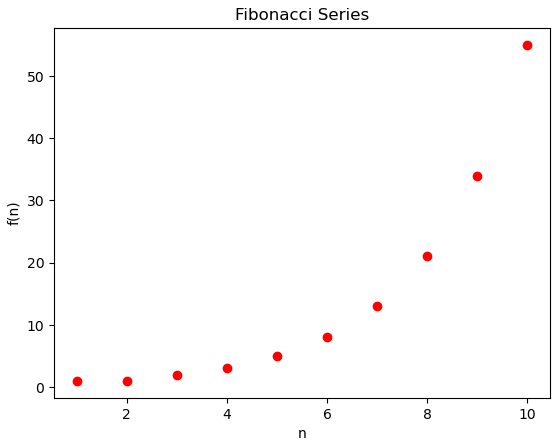
\includegraphics[width=0.5\textwidth]{./chapters/ch-python/figures/fib_exp.png}
\caption{Plot Fibonacci series as scatter plot.}
\label{fig:fib_exp}
\end{figure}

The presentation of the plot can be customized. For example, use \verb|plt.xlim(x1, x2)|, \verb|plt.ylim(y1, y2)| to change the axis limitations, etc. It is possible to change curve color, size, style, and marker size, style, etc.

\subsection{Seaborn}

Seaborn is another visualization library built on top of the Matplotlib library. It tries to standardize the plots with a simple function call. It scarifies some flexibility that Matplotlib offers, but makes plotting easier.

An example of using Seaborn to plot a histogram is given below. The result is given in Fig. \ref{fig:normhistexp}.
\begin{lstlisting}[language=Python]
import numpy as np
import pandas as pd
import matplotlib.pyplot as plt
import seaborn as sns

x = np.random.randn(1000)
plt.figure()
sns.histplot(x, color="red")
plt.title("Histogram Example")
plt.xlabel("x")
plt.ylabel("Count")
\end{lstlisting}

\begin{figure}[htbp]
	\centering
	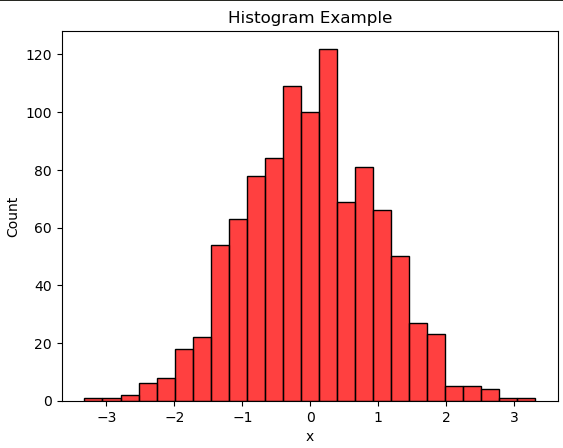
\includegraphics[width=0.5\textwidth]{./chapters/ch-python/figures/normhistexp.png}
	\caption{Histogram plot using Seaborn.}
	\label{fig:normhistexp}
\end{figure}

An example of using Seaborn to plot a count plot for discrete values (usually category values) is given below. Notice that the attribute whose values are put into categories is assigned to $x$ of \verb|seaborn.countplot()|. The result is given in Fig. \ref{fig:countplot}.
\begin{lstlisting}[language=Python]
import numpy as np
import pandas as pd
import matplotlib.pyplot as plt
import seaborn as sns

response = ["yes", "no", "no", "yes", "yes", "yes", "yes", "yes", "yes", "no", "yes", "yes", "NA", "NA"]
plt.figure()
sns.countplot(x=response, color="blue")
plt.title("Count Plot Example")
plt.xlabel("response")
plt.ylabel("Count")
\end{lstlisting}

\begin{figure}[htbp]
	\centering
	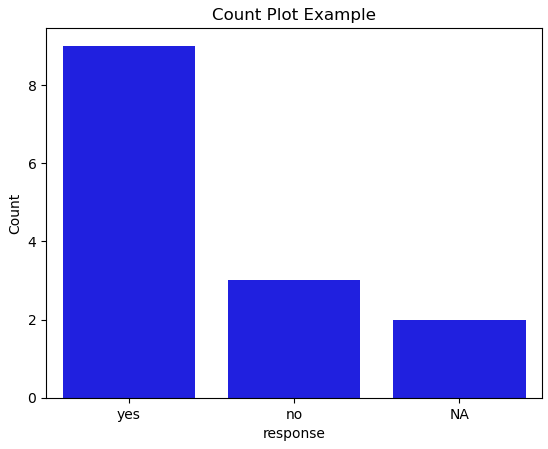
\includegraphics[width=0.5\textwidth]{./chapters/ch-python/figures/countplotexp.png}
	\caption{Count plot using Seaborn.}
	\label{fig:countplot}
\end{figure}

Bot plot gives the maximum, minimum, and interquartile range (IQR) of the data. In the box plot, the data is split into 4 parts, namely $x<Q_1$ ($0\%-25\%$), $Q_1<x<Q_2$ ($25\%-50\%$), $Q_2<x<Q_3$ ($50\%-75\%$), and $Q_3<x$ ($75\%-100\%$). The IQR gives the range between $Q_1$ and $Q_3$, i.e., the half in the middle $25\%-75\%$. An example is given below. The result is given in Fig. \ref{fig:boxplot}.
\begin{lstlisting}[language=Python]
import numpy as np
import pandas as pd
import matplotlib.pyplot as plt
import seaborn as sns

x = np.random.randn(1000)
plt.figure()
sns.boxplot(x, color="blue")
plt.title("Box Plot Example")
plt.xlabel("Input")
plt.ylabel("Value")
\end{lstlisting}

\begin{figure}[htbp]
	\centering
	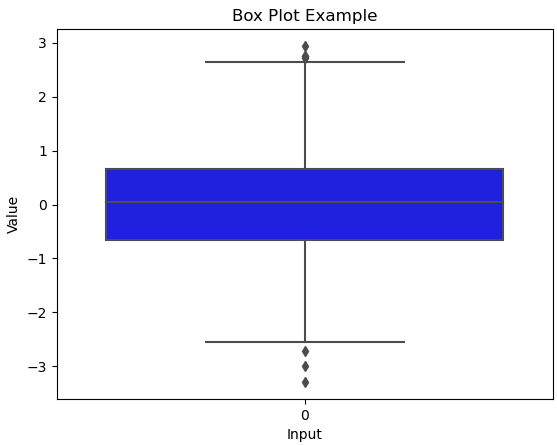
\includegraphics[width=0.5\textwidth]{./chapters/ch-python/figures/boxplotexp.png}
	\caption{Box plot using Seaborn. The box gives IQR. The bars below and above the box give $Q_1-1.5\times\textup{IQR}$ and $Q_3+1.5\times\textup{IQR}$, respectively. The dots are outliers.}
	\label{fig:boxplot}
\end{figure}

There are many more plot functions in Seaborn. For example, scatter plot \verb|seaborn.scatterplot()| works similar with Matplotlib as shown by Fig. \ref{fig:fib_exp}. The marker size and color can be adjusted to reflect different parameters, just like in R language. Pairplot \verb|seaborn.pairplot()| generates a matrix of plots to demonstrate associations of columns in a data frame.
